En la sección \ref{seccion7} dimos una idea general de lo que se entiende por una trenza. Veamos su definición más formal:\\

\underline{\textbf{Definición:}}\\
Consideremos el cubo $\mathds{D} = \{(x,y,z) / 0 \leq x,y,z \leq 1\}$ y situamos $A_{i}$ puntos en su cara superior y $B_{i}$ puntos en la cara inferior, siendo $i \in \mathds{N}$. Podemos considerar dichos puntos como \\
$A_{1}=(\frac{1}{2},\frac{1}{n+1},1)$, $A_{2}=(\frac{1}{2},\frac{2}{n+1},1)$,...,$A_{n}=(\frac{1}{2},\frac{n}{n+1},1)$, \\ $B_{1}=(\frac{1}{2},\frac{1}{n+1},0)$, $B_{2}=(\frac{1}{2},\frac{2}{n+1},0)$,...,$B_{n}=(\frac{1}{2},\frac{n}{n+1},0)$.\\
  Unimos cada punto $A_{i}$ con un cierto punto $B_{k}$, $i, k \in \mathds{N}$, mediante arcos poligonales simples $d_{i}$ de modo que:
\begin{enumerate}
	\item $ d_{1}, d_{2},...,d_{n} $ sean disjuntos.
	\item Los arcos $ d_{i} $ no pueden conectar puntos $A_{i}$ o $B_{i}$ entre sí.
	\item Al cortar por cualquier plano horizontal, cada arco $ d_{i} $ toca en un sólo punto al plano. 
\end{enumerate}
A cada uno de estos arcos poligonales $ d_{i} $ les llamaremos \textbf{cadena}s y al conjunto de las n-cadenas se le conoce como \textbf{trenza}. Podemos ver algunos ejemplos de trenzas en la figura \ref{tren1}.
\begin{figure}[h!]
	\centering
	\subfigure[]{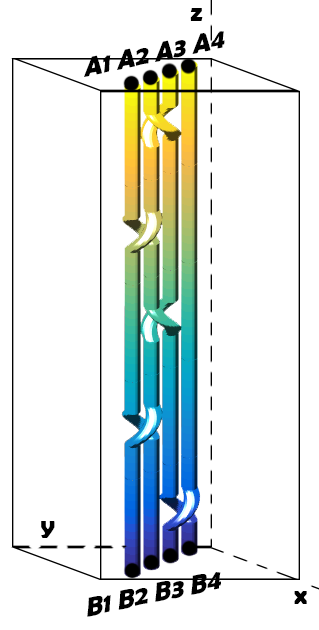
\includegraphics[width=3cm]{itrenzas/t1cubo.png}}
	\space
	\subfigure[]{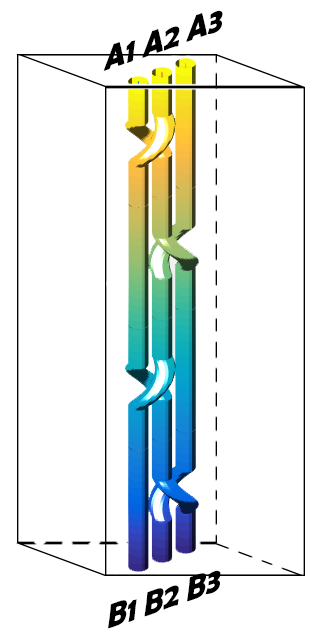
\includegraphics[width=2.9cm]{itrenzas/t2cubo.png}}
	\caption{Ejemplos de trenzas}
	\label{tren1} 
\end{figure}  

Anteriormente vimos que a cada trenza le corresponde un nudo o un enlace particular. Se obtendrá uniendo los extremos superiores con los extremos inferiores de las cadenas en el mismo orden. A este nudo se le conocerá como \textbf{trenza cerrada}.\\
Denotaremos como $\mathscr{B}_{n}$ al conjunto de todas las trenzas de n cadenas.\\

\section{Fundamentos.}
\begin{centering}
	\subsection{Equivalencia de trenzas:}
\end{centering}

Intuitivamente diremos que dos trenzas son equivalentes si podemos deformar las cadenas de las trenzas de forma que ambas trenzas se vean iguales. Las trenzas de la figura \ref{tren3} son equivalentes.
\begin{figure}[h!]
	\centering
	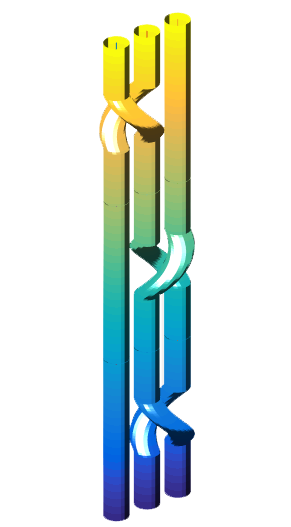
\includegraphics[width=4cm]{itrenzas/t3.png}
	\space
	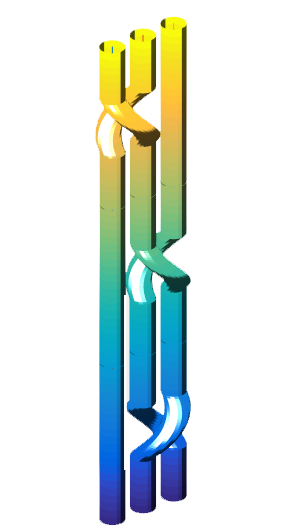
\includegraphics[width=4cm]{itrenzas/t4.png}
	\caption{Trenzas equivalentes.}
	\label{tren3} 
\end{figure}

\textbf{\underline{Definición:}}\\
Consideremos la cadena $d$ de una trenza situada en el cubo $\mathds{D} = \{(x,y,z) / 0 \leq x,y,z \leq 1\}$. Podemos quedarnos con una representación poligonal de las cadenas de la trenza. \\
Sea AB un segmento de dicha cadena y C un punto en el cubo de forma que el triángulo $\triangle ABC$ no corta a ninguna otra cadena de la trenza y sólo toca a la cadena $d$ en el segmento AB. Supongamos además que los segmentos AC y CB cortan a cualquier plano horizontal del cubo en un sólo punto como mucho. Visualizamos estas condiciones en la primera imagen de la figura \ref{elem}.\\
Bajo estas condiciones definimos un \textbf{movimiento elemental} como la operación $ \Omega $ que intercambia el segmento AB por los segmentos AC $ \cup $ CB.\\

La operación inversa $ \Omega^{-1} $ que intercambia los segmentos AC $\cup$  CB, que formen parte de una cadena, por el segmento AB de forma que el triángulo $\triangle ABC$ no corte a ninguna otra cadena, también es considerada un movimiento elemental. \\
Podemos ver la representación de ambos movimientos en la figura \ref{elem}.\\
\begin{figure}[h!]
	\centering
	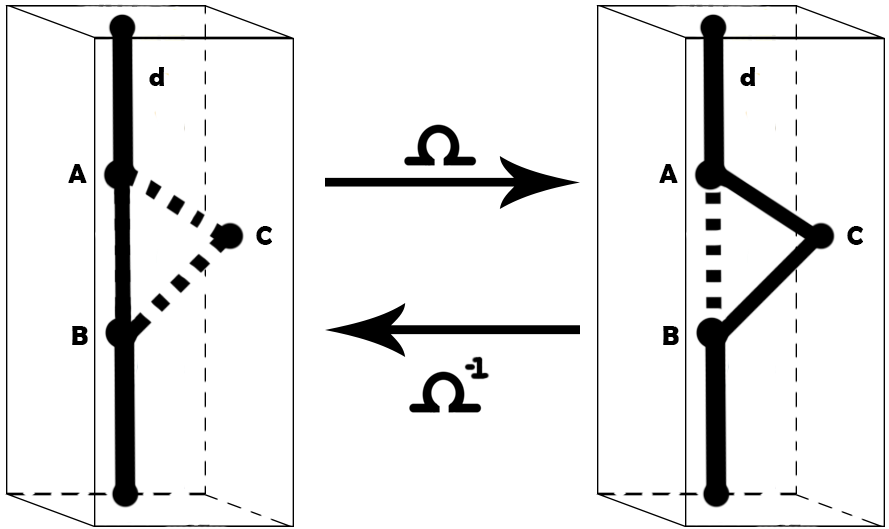
\includegraphics[width=8.5cm]{itrenzas/elemental.png}
	\caption{Movimiento elemental}
	\label{elem} 
\end{figure}


\textbf{\underline{Definición 2.1:}}\label{defequi}\\
Sean dos trenzas $\beta$, $\beta'$. Diremos que son \textbf{equivalentes} ($\beta \sim \beta'$) si existe una cadena finita de trenzas $ \beta = \beta_{0}$, $\beta_{1},...,\beta_{m}=\beta'$ tal que cada par de trenzas $ \beta_{i}, \beta_{i+1}, i=0,..,m-1, $ está relacionado por un movimiento elemental. A esta cadena de trenzas equivalentes la representaremos del siguiente modo:
\begin{center}
	$ \beta = \beta_{0} \rightarrow \beta_{1} \rightarrow ... \rightarrow \beta_{m}=\beta'$
\end{center}

Si dos trenzas $\beta$, $\beta'$ no son equivalentes, lo denotaremos como $\beta \not \sim \beta'$.\\

Denotaremos como $ \textbf{B}_{n} $ al conjunto de todas las trenzas de n cadenas no equivalentes entre sí. Es decir, ${B}_{n}$ = $\mathscr{B}_{n}$/$ \sim $.\\

\bigskip
\begin{center}
	\subsection{Proyección de una trenza.}
\end{center}
Consideremos una trenza situada en el cubo $\mathds{D} = \{(x,y,z) / 0 \leq x,y,z \leq 1\}$. Podemos obtener la proyección de la trenza sobre el plano-yz haciendo la proyección  p(x,y,z) = p(0,y,z) de cada uno de los puntos de la misma. De este modo visualizaremos las cadenas como curvas poligonales simples sobre el plano-yz.\\

Haciendo uso de movimientos elementales, podemos obtener trenzas equivalentes a la inicial de modo que cualquier intersección que vemos en su proyección sea producida por sólo dos cadenas y en un sólo punto. Además podemos obtener trenzas equivalentes tales que las intersecciones de las cadenas se sitúen en distintos niveles. De modo que dada una trenza cualquiera, nos quedaremos con su trenza equivalente cuya proyección cumpla estas condiciones. Podemos ver un ejemplo de cómo obtener una proyección de una trenza en la figura \ref{impers}.\\ 

\begin{figure}[h!]
	\centering
    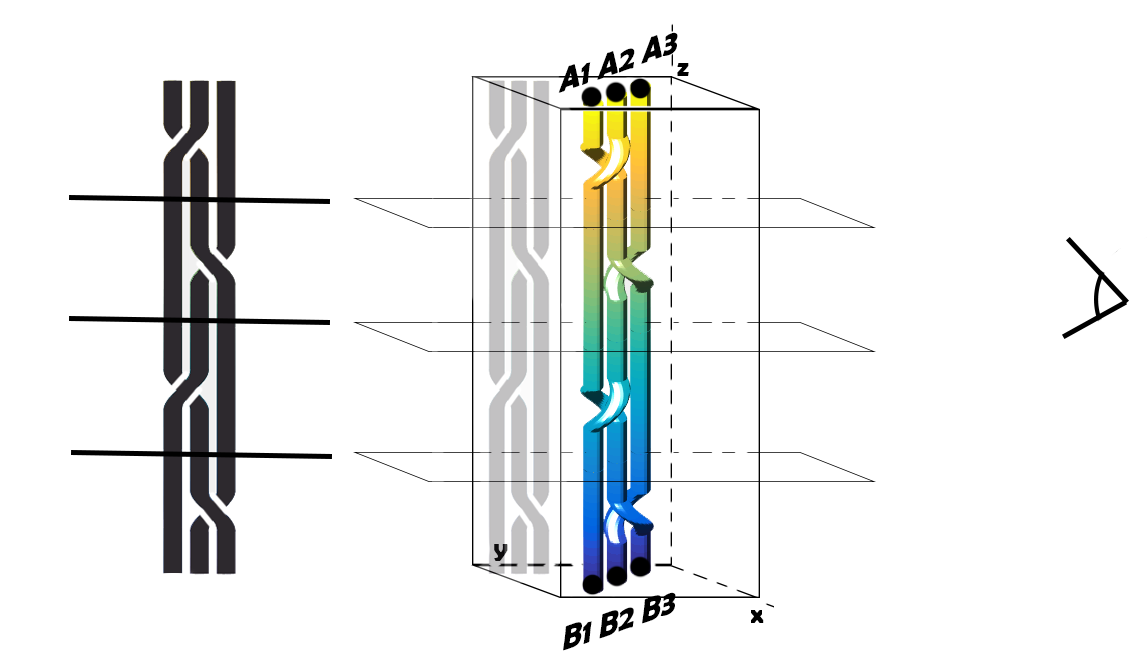
\includegraphics[width=15cm]{itrenzas/pers.png}
	\caption{Proyección de una trenza}
	\label{impers} 
\end{figure}

En la figura \ref{tren2} se pueden ver las proyecciones de las trenzas representadas en la figura \ref{tren1}.\\
\begin{figure}[h!]
	\centering
	\subfigure[]{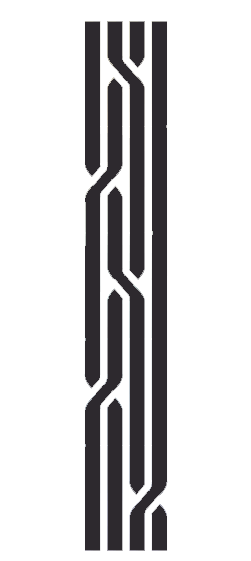
\includegraphics[width=2.7cm]{itrenzas/t1pro.png}}
	\space
	\subfigure[]{
\includegraphics[width=2.3cm]{itrenzas/t2pro.png}}
	\caption{Proyección de trenzas}
	\label{tren2} 
\end{figure} 

\newpage
\begin{center}
	\subsection{Notación de trenzas:}
\end{center}
Para poder trabajar de forma cómoda con las trenzas vamos a darle la siguiente notación:\\

Supongamos que disponemos de una trenza y de su proyección. Recordemos que modificamos la trenza con movimientos elementales de modo que en cada plano horizontal que corta imaginariamente a la trenza sólo podemos tener dos cadenas que intercambien sus posiciones generando así la intersección que vemos a cierto nivel en la proyección. Vamos a quedarnos con estas secciones de cadenas que producen la intersección en la proyección.\\  

Consideremos que estos segmentos de cadenas unen las posiciones $i$ con la $i+1$ y las posiciones $i+1$ con la $i$. Al producir un intercambio de posiciones de estos segmentos se producirá un \textbf{cruce}, que se verá como la intersección de cadenas en la proyección de la trenza.\\
Este cruce puede realizarse de dos formas: 
\begin{itemize}
	\item El segmento que parte de la posición $i$ cruza por delante al segmento que inicialmente parte en la posición $i+1$. En este caso el cruce se denota como $\sigma_{i}^{-1}$ y se conoce como un cruce negativo.
	\item  El segmento que parte de la posición $i$ cruza por detrás al segmento que inicialmente parte en la posición $i+1$. En este caso el cruce se denota como $\sigma_{i}^{+1}$ o simplemente $\sigma_{i}$ y se conoce como un cruce positivo.
\end{itemize}
Podemos verlo más claro en la figura \ref{tren4}.\\
\begin{figure}[h!]
	\centering
	\subfigure[$\sigma_{i}^{-1}$]{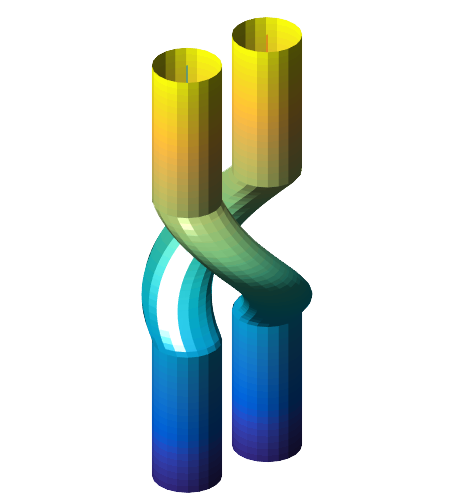
\includegraphics[width=2cm]{itrenzas/t5.png}}
	\space
	\subfigure[$\sigma_{i}$]{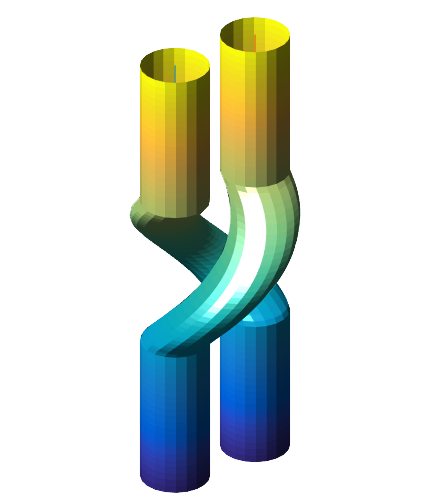
\includegraphics[width=2cm]{itrenzas/t6.png}}
	\caption{Signo cruce.}
	\label{tren4} 
\end{figure}

La \textbf{n-trenza trivial} se define como la n-trenza que no realiza ningún cruce. La denotaremos como $1_{n}.$ \\

Cualquier trenza no trivial tendrá de una serie de cruces. En cada plano horizontal podremos tener como mucho un cruce. Notaremos a la trenza con la secuencia de cruces que tenga, empezando por la parte superior de la trenza. A esta secuencia se le conoce como \textbf{palabra} que representa a la trenza. Podemos ver un ejemplo en la figura \ref{tren5}.\\
\begin{figure}[h!]
	\centering
	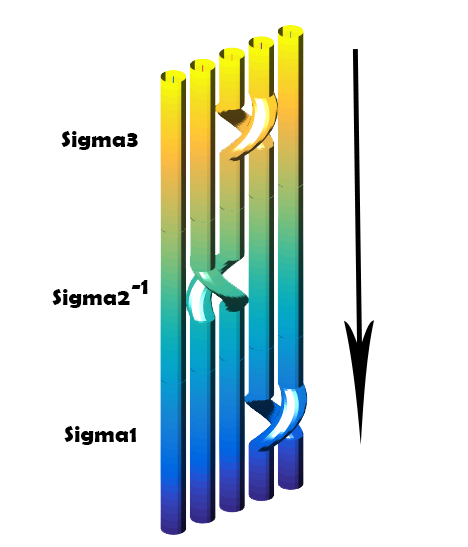
\includegraphics[width=5cm]{itrenzas/t7.png}
	\caption{Trenza $\sigma3\sigma2^{-1}\sigma4$.}
	\label{tren5} 
\end{figure}


